Low energy electron diffraction (LEED)\index{LEED} is a technique for the determination of surface structures. It uses an electron beam $0.5mm$ with low energies ($\leq \SI{500}{\eV}$) which is scattered from the surface and creates an diffraction pattern. The shape of this pattern is then related to the surface geometry. Note that although a sharp LEED diffraction pattern may be observed, the area of coherently scattering electrons is about \SI{20}{\nm}. Thus a small region on the illuminated sample has to be ordered in order to show diffraction patterns. This does not mean that the whole sample is ordered.

% It may be used qualitatively to determine orientation and size of an absorbat with respect to the substrate by the position of the diffraction spots\cite{tang_growth_2002}. It is also suitable to gain accurate information on elevation and rotation angles of surface grains\cite{kraus_towards_2013} and corrugation amplitudes.

Lets us first consider an easy model. Electrons from the gun penetrate the sample surface and interact with the solid. Where the interaction is not important one may consider an exponential decay in direction of propagation:
$$I(d)=I_0\cdot e^{-\frac{d}{\Lambda(E)}}$$ where $I$ is the intensity in penetration depth d and $\Lambda(E)$ is the inelastic mean free path of electrons. It depends on their energy E, but is not so sensitive to the material itself in this energy range. It is typically between \SIrange{5}{20}{\angstrom} for energies \SIrange{20}{200}{\eV}. This is why LEED is more surface than bulk sensitive.

\subsection{Single (elastic) scattering theory}\index{LEED!elastic scattering}
As electrons are particle and wave at the same time, they have a \index{de Broglie} de Broglie wave length $\lambda$:
$$\lambda=\frac{h}{\sqrt{2mE}} \qquad \lambda[nm] \approx \sqrt{\frac{1.5}{E[eV]}}$$
Considering a real space lattice {$\vec a_1,\vec a_2,\vec a_3$}, scattering is described in reciprocal lattice more conveniently. Transforming the basis set $\vec a_i$ to its corresponding reciprocal basis set 
$$\vec k_i=\frac{2\pi \vec a_{i+1}\times\vec a_{i+2}}{\vec a_i\cdot(\vec a_{i+1}\times \vec a_{i+2})}$$ with $a_i \in [0,1,2,3]$.
The Laue condition (Bragg's theorem in reciprocal space) $$\vec k-\vec k_0 = \vec G_{hkl}$$ with $$\vec G_{hkl}=h\vec k_1+k\vec k_2+l\vec k_3$$ describes conditions for an incident beam $\vec k_0$ and its diffracted equivalent $\vec k$. Remember that the penetration depth is so small, that there are only enough contributing scattering partners for directions parallel to the surface. Therefore Laue's condition reduces to surface parallel ($\parallel$) components of $\vec k$ $$\vec k^{\parallel}-\vec k^{\parallel}_0=\vec G_{hk}=h\vec k_1 + k \vec k_2$$ To visualize the possible diffraction conditions of a surface one can use the Ewald's sphere construction.
\paragraph{Ewald's sphere}\index{LEED!Ewald's sphere}
By depicting the surface as an infinitely extended 2D-array of dots separated by $h\vec k_1$ in one and by $k\vec k_2$ in the other direction, one chooses an incident beam $k_0$. It is drawn such that it ends on the reciprocal lattice plane. Then one draws a circle around this point with radius $r=|k_0|$ (energy conservation). Now extend the reciprocal lattice points of the surface to rods perpendicular to the surface. Every vector from the origin of the circle and the intersection of circle and rod is an allowed diffracted beam. 

When increasing the energy, the radius $|\vec k_0|$ more and more rods contribute and get visible on the screen. If the energy is high enough, one can see the high order laue zone where diffraction spots form a dense ring-shaped feature.
\begin{figure}[h!]\label{ewald-sphere}
 \centering
 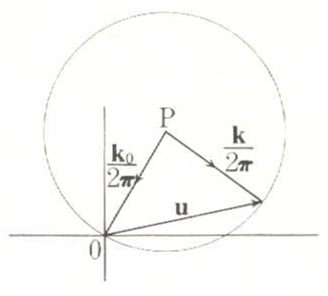
\includegraphics[height=6cm]{./images/ewald-sphere.jpg}
 \caption{ewald-sphere, ``top'' view, taken from \cite[109]{cowley_diffraction_1981}}
\end{figure}

\begin{figure}[h!]\label{LEED}
 \centering
 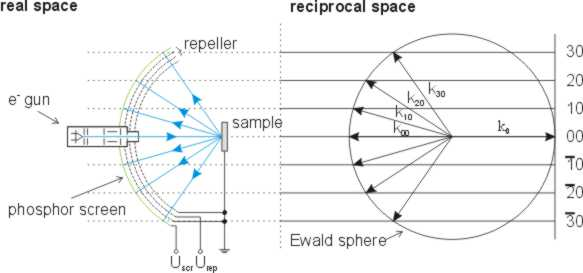
\includegraphics[height=6cm]{./images/ThreeGridLeed.jpg}
 \caption{ewald-sphere, ``side'' view, taken from \cite{threegridleed.jpg_2015}}
\end{figure}

For electrons with energies of \SI{0.04}{\eV} the diameter of the ewald sphere will be \SI{50}{\per \angstrom} in reciprocal space f. On this sphere only a small region of radius \SI{5}{\per \angstrom} will contain the small angle scattered waves of LEED.

\paragraph{Structure factor}\index{LEED!Structure factor}
Consider a function that describes the atomic positions in real space $\phi(\vec r)$. Let it be integrable, when one defines the Fourier transform such that 
\begin{equation}\label{eq:structure_factor}
\phi(\vec k)=\int_{\vec r} \phi(\vec r)e^{-i\vec k \vec r}d\vec r 
\end{equation}
If one chooses $\phi(\vec r)$ to resemble the form of the scatter partners as well - like $\phi(\vec r)=f(\vec r)\circ \sum_{j=1}^N\delta(r-R_j)$ where $R_j$ are the atom positions in real space and $f(r)$ describes the form of the atom. $\circ$ shall represent the convolution product, i.e. $FT(\phi(\vec r))=\phi(\vec k)=f(\vec k)\cdot \sum_{j=1}^N e^{-i\vec k \vec R_j}$ As the intensity $I(\vec k)\varpropto |\phi(\vec k)|^2$
$$\langle I(\vec k) \rangle \varpropto 
\langle |\phi(\vec k)|^2 \rangle =
\langle |f(\vec k)|^2 \left( \sum_{m=1}^N e^{-i\vec k \vec R_m} \right) \left( \sum_{n=1}^N e^{i\vec k \vec R_n}
\right) \rangle=|f(\vec k)|^2 \underbrace{\langle \left( \sum_{m,n=1}^N e^{i\vec k (\vec R_n-\vec R_m)} \right) \rangle }_{S(\vec k)}$$

One can calculate different structure factors for different lattices. As used crystals are fcc lattices, their basis set $R_j$ is 
$$ \vec{R}_0 = \vec{0} \quad
 \vec{R}_1 = (a/2)(\vec{a_1} + \vec{a_2})\quad
 \vec{R}_2 = (a/2)(\vec{a_2} + \vec{a_3})\quad
 \vec{R}_3 = (a/2)(\vec{a_1} + \vec{a_3})$$ with indices given by (1/2,1/2,0), (0,1/2,1/2), (1/2,0,1/2).

Following the definition of \eqref{eq:structure_factor} above, one gains an relation of $\vec {k}=(h,k,l)^T$ that describes the structure factor. Exchanged $\vec k$ with $\vec q$ in the calculation for clarity.
\begin{align*}
S_{\vec{q}} &=  f \left[ e^{-i\vec{q}\cdot\vec{0}} + e^{-i\vec{q}\cdot(a/2)(\vec{a_1} + \vec{a_2})} + e^{-i\vec{q}\cdot(a/2)(\vec{a_2} + \vec{a_3})} + e^{-i\vec{q}\cdot(a/2)(\vec{a_1} + \vec{a_3})} \right] \\
&= f \left[ 1 + (-1)^{h + k} + (-1)^{k + l} + (-1)^{h + l} \right] \\
&=  \begin{cases} 4f &\mbox{h,k,l all even or all odd}\\
                  0 &\mbox{mixed parity} \end{cases}
\end{align*}
This means, that only diffractions with $S_{\vec q}\neq 0$ contribute to the diffraction pattern. For fcc lattices, only sets of all even or all odd (h,k,l) create the pattern. 

For bcc its $$ \vec{R}_0 = \vec{0} \quad
 \vec{R}_1 = (a/2)(\vec{a_1} + \vec{a_2}+ \vec{a_2})$$ and thus 
 $$(h,k,l)=\begin{cases} 2f &\mbox{h,k,l all even}\\
                  0 &\mbox{h,k,l all odd} \end{cases}$$ due to the different basis.

In general, the structure factor is a imaginary quantity. It has the form $S(\vec k)=F_{hkl}e^{-i\alpha_{hkl}}$. $F_{hkl}$ describes the super-positioned amplitudes, while $\alpha_{hkl}$ is the phase of the resulting scattered wave. One can think of it, like having the same atoms on a crystal plane (hkl) scattering the incoming wave, with the same amplitude for each equal atom and the same phase. Now consider a parallel plane (hkl) with the same plane distance but occupied with another set of the same atoms. Since these planes are parallel Braggs law is fulfilled, the incident wave gets scattered but with a phase shift that depends on the two plane's separation. The structure factor takes these planes into account and adds the two scattered waves into one. Since these planes are created by the basis of the crystal, one just needs to know the single atom's distance to the initial plane (arbitrarily chosen atom, mostly $\vec 0$) to calculate the structure factor. If atoms are not the same, i.e. their scattered amplitude is not the same, the structure factor adapts with different $f_i$'s for different atomic species. Further reading into computational efforts and such can be done in ref. \cite{van_hove_surface_1979}.

Further reading into determining overlayer distances and structure of S on Ni can be found here \cite{demuth_small_1973,duke_structure_1973,andersson_surface_1972}
\paragraph{Temperature correction}\index{Debye-Waller factor}
Corrections have to be made if thermal motion is included. A solid with temperature $T$ has some kinetic energy which makes the atoms able to oscillate around their central position $R_j$. If one replaces $R_j$ in the calculation above with some time dependend value $\vec r_i(t)=\vec r_{i,0}+\vec u_i(t)$, with fast changing function $u(t)$ describing the dislocation from the ideal position, one yields:
$$ \langle S(\vec q) \rangle =\sum_{i}f_{i}\,\langle\exp\left[i\,\vec{q}\cdot\left(\vec{r}_{i.0}+\vec{u}_{i}(t)\right)\right]\rangle=\sum_{i}f_{i}\,\exp\left[i\,\vec{q}\cdot\vec{r}_{i.0}\right]\,\langle\exp\left[i\,\vec{q}\cdot\vec{u}_{i}(t)\right]\rangle $$
Expanding the exponential function to terms $\leq 2^{nd}$ order 
$\langle \exp\left[i\,\vec{q}\cdot\vec{u}_{i}(t)\right] \rangle \approx 1+i\,\langle \vec{q}\cdot\vec{u}_{i}(t)\rangle-\frac{1}{2}\langle\left(\vec{q}\cdot\vec{u}_{i}(t)\right)^2\rangle$ where the first term equals zero because $\langle \vec{u}_i(t)\rangle=0$ (vibration around center).

$$\langle \left(\vec{q}\cdot\vec{u}_{i}(t)\right)^2 \rangle=|\vec{q}|^{2}\,\langle|\vec{u}_{i}(t)|^2\rangle \,\langle\cos^{2}\theta\rangle$$ The time avarage 
$$ \langle \cos^{2}\theta \rangle=\frac{\int_{0}^{2\pi}\mathrm{d}\phi\int_{0}^{\pi}\mathrm{d}\theta\,\sin\theta\cos^{2}\theta}{\int_{0}^{2\pi}\mathrm{d}\phi\int_{0}^{\pi}\mathrm{d}\theta\,\sin\theta}=\frac{1}{3} $$ inserted into the expansion results in
$$\langle \exp\left[i\,\vec{q}\cdot\vec{u}_{i}(t)\right]\rangle \approx1-\frac{1}{6}\,|\vec{q}|^{2}\,\langle|\vec{u}_{i}(t)|^2\rangle \approx \exp\left[-\frac{1}{6}\,|\vec{q}|^{2}\,\langle|\vec{u}_{i}(t)|^2\rangle \right]$$
Put it in the definition of $\langle S(\vec q) \rangle$ results in
$$\langle S(\vec q) \rangle =\underbrace{\sum_i f_{i}\,\exp\left[i\,\vec{q}\cdot\vec{r}_{i,0}\right]}_{S_0(\vec q)}\,\exp\left[-\frac{1}{6}\,|\vec{q}|^{2}\,\langle|\vec{u}_{i}(t)|^2 \rangle \right]$$
Time averaging the intensity yields $$\langle I \rangle \propto \langle S(\vec q)\rangle^2 =S_0^2(\vec q)\,\exp\left[-\frac{1}{3}\,|\vec{q}|^{2}\,\langle|\vec{u}|^2\rangle \right]=I_{0}\underbrace{\exp\left[-\frac{1}{3}\,|\vec{q}|^{2}\,\langle|\vec{u}|^2\rangle \right]}_{DWF}$$
\begin{itemize}
 \item This means the higher the amplitude of displacements (higher T), the weaker the overall intensity of the spots. This is consistent with the idea that the higher the temperature, the lower the coherence between two areas. This reduces the intensity.
 \item The DWF reduces the intensity for peaks $|\vec q|>0$ so that peaks with high $|\vec q|$ have less intensity than those with small $|\vec q|$. For initial reading and detailed calculations see \cite{debye_interferenz_1913}.
\end{itemize}
The attenuation of intensity from the DWF can be used to investigate oscillating dislocations of surface atoms. As one would expect the kinetic energy from a vibration with force constant D (harmonic oscillator) to be $D\langle u^2\rangle$, its thermal energy is $k_bT$. When now the atom faces a missing surface layer (and therefore becoming itself one) the atoms left to share energy with lie in the same plane or below. It one assumes pairwise interaction one would expect $D$ to be halfed or $\langle u^2 \rangle$ compared to a intact pair of atoms\cite[69]{woodruff_modern_1986}. Although vibrations may be accessible in LEED it is not well suited to address this question. As other studies indicate the effect of enhanced amplitudes is most dominant at the very surface and - due to the fact that LEED probes several layers - it may average $\langle u^2 \rangle$ over the first 3-5 layers.

One may look deeper into what causes scattering when electrons face atoms. The coulomb interaction is strong and electrons get scattered depending on the electron density of the atom. So if one knew both the amplitude and the phase of the scattered electrons, one could calculate the electron densities. Since the phase can not be obtained a workaround has to be chosen such that one has a relative measurement of the in- and outcoming phases. If one adds an electronically denser item (like a metal atom) in the crystal it will change the diffraction pattern and one may derive the phases from that. Same is done with molecules, where one compares an already resolved scattering pattern with the ``new'' one to track changes and calculate the phase.

Another (quantum mechanical) description can be found in \cite[341]{liuksiutov_two-dimensional_1992}.

\paragraph{Spot shapes and changes} to them are given in \cite[36]{woodruff_modern_1986}, along with a detailed error evaluation. It describes under witch condition peak splitting may occur and gives examples for peak splitting related to domain boundaries and different atomic ordering on surfaces. If the surface is made of vicinal steps (i.e. 100 steps with 111 terraces, like 532) one can see 
\begin{itemize}
 \item The lattice of the substrate (in this case the unit cell contains the step distance and height)
 \item Splitted LEED spots which arise from the kinked surface and the periodic defect step formation on the ctystal\cite[37ff]{riemann_ionic_2002}.
\end{itemize}

\paragraph{Friedel's law}\cite[93]{cowley_diffraction_1981}
Provided that for the electrons no absorption effect is important, the electron desity $\rho(\vec r)$ may be assumed to be a real function satisfying \begin{align}
F(-\vec u) &= \int \rho(\vec r) \exp{[2\pi i(-\vec u)\vec r]} d\vec r \\                                                                                                                                                      &=F^\star(\vec u)                                                                                                                                                      \end{align}
As the intensities scale with $I=|F|^2$ it follows that inversion of a crystal through a center of symmetry does not change the diffraction intensities in a kinematic (single scattering) approximation. Since the inversion of \eqref{eq:structure_factor} gives the electron density $$\rho(r)=\int F(\vec u)\exp{[-2\pi \vec u \vec r]} d\vec u$$ If the diffraction amplitudes could be measured so that $F(\vec u)$ could be derived, than $\rho (\vec r)$ can be calculated by evaluating the integral numerically. But measurement of the wave amplitudes $F(\vec  u)$ is not possible, only the intensities $FF^*$ are recorded. Thus information on the phases is lost and $\rho(\vec r)$ not calculable.

\paragraph{superstructure determination}
\underline{\ \ \ \ \ \ \ \ asd \ \ \ \ \ \ \ \ \ }
\subsection{Multiple scattering theory}See \cite[55]{woodruff_modern_1986} for concepts of modeling, \cite{van_hove_surface_1979} for explaining the calculations.

The incident beam of coherent (waves have equal phases) electrons are diffracted under the fulfillment of Laue's law to result in coherent radiation on the LEED screen. Above only single scattering event were taken into account but the interaction of electrons and solid is much more pronounced than for example for X-rays. So electrons scattered once will be able to scatter a second or third time, following again Laue's law. This implies scattering on the very same oriented crystal planes. Then the phases are uniquely defined and the waves amplitudes are added. This is referred to as ``dynamical'' scattering. So if the crystal has some impurities, grain-boundaries and such, scattered electrons will be attenuated. Multiple scattering therefore gives an indication on the purity of the crystal itself. On the other hand, if atomic ordering does not extend over areas required for defined scattering the relative phases of each ordered crystal domain will add up randomly and their amplitudes are added incoherently. This is referred to as ``multiple elastic scattering''.

As a comparison, the path length for X-rays to be scattered multiple times is $\approx \SI{1}{\micro \meter}$, serveral times longer for neutrons and only one or two hundert \si{\angstrom} for eletrons\cite[90]{cowley_diffraction_1981}.

\paragraph{Resolution and difficulties}
I real world experiments, there is often a spread in incoming wave momenta and the problem of focus. 
\textbf{Finite Sources - Ewald shell emergence}
For LEED witch magnetic focus, the angle of convergence may be chosen as high as \SI{E-3}{\radian}(within magnetic lenses of an tunneling electron microscope). But even within this small range of angles, the appearance of the Ewald sphere changes. If one chooses two different angles for incoming waves $\vec k_0$ the waves scatter in different directions resulting in a blurring of diffraction spots.

\paragraph{Wavelength spread}
For electrons a nearly monochromatic radiation with line widths of about $10^{-6}\lambda$ are achieveable (1981). The spread of wavelengths in the incoming beam modifies the length of the $\vec k_0$ and as a result the diffracted spot shapes change from spots to lines variing as well in orientation as in length\cite[113]{cowley_diffraction_1981}``being small and parallel to $\vec k_0$ in the limit of small scattering angles; of medium length and roughly perpendicular to $\vec k_0$ like for intermediate scattering angles and of maximum length and oppositely directed to $\vec k_0$ for scattering angles of \SI{180}{\degree}''.

Adding this effect to the finite source problem, one ends in a complicated scattering volume. Thus the relationship of the observed intensity to the function $|F(\vec q)|^2$ is only to derived by calculation from a detailed model containing the parameters of the experimental system.

For some examples of vacancy deviations, see \cite[144-151]{cowley_diffraction_1981}.
In LEED, if the size of diffraction elements are smaller than the width of the transfer function, one observes broadening in the peaks and therefore makes it able to access their size\cite[40]{liuksiutov_two-dimensional_1992}.

